\documentclass[12pt,a4paper]{article}
\usepackage[utf8]{inputenc}
\usepackage[spanish,es-tabla]{babel}
\usepackage{geometry}
\usepackage{graphicx}
\usepackage{multirow}
\usepackage{tabularx}
\usepackage{mathptmx}
\usepackage{fancyhdr}
\usepackage{array}
\usepackage[table]{xcolor}
\usepackage{titlesec}
\usepackage{setspace}
\usepackage{microtype}
\usepackage{lastpage}
\usepackage{booktabs}
\usepackage{enumitem}
\usepackage{amsmath}
\usepackage{amsfonts}
\usepackage{amssymb}

\usepackage{float}
\usepackage{placeins}
\usepackage{tikz}
\usepackage{pgfplots}
\pgfplotsset{compat=1.17}
\usetikzlibrary{arrows.meta,positioning,shapes.geometric,calc}

\graphicspath{{images/}{../images/}{./}}

\geometry{
    top=4.7cm,
    bottom=2.5cm,
    left=2.5cm,
    right=2.5cm,
    headheight=3.9cm,
    headsep=0.4cm
}

\setstretch{1.15}
\setlength{\parindent}{0pt}
\setlength{\parskip}{0.45em}
\setlength{\tabcolsep}{4pt}

\titleformat{\section}
  {\normalfont\fontsize{12}{14.5}\bfseries}{\thesection.}{0.6em}{\uppercase}
\titlespacing*{\section}
  {0pt}{1.8ex plus 0.4ex minus 0.2ex}{0.6ex plus 0.2ex}

\titleformat{\subsection}
  {\normalfont\fontsize{11.5}{13.5}\bfseries}{\thesubsection.}{0.5em}{}
\titlespacing*{\subsection}
  {0pt}{1.4ex plus 0.3ex minus 0.1ex}{0.4ex plus 0.1ex}

\titleformat{\subsubsection}
  {\normalfont\fontsize{10.5}{12.5}\bfseries\itshape}{\thesubsubsection.}{0.4em}{}
\titlespacing*{\subsubsection}
  {0pt}{1.1ex plus 0.2ex minus 0.1ex}{0.3ex plus 0.1ex}

\newcolumntype{Y}{>{\centering\arraybackslash}X}
\newcolumntype{L}{>{\raggedright\arraybackslash}X}
\newcolumntype{C}{>{\centering\arraybackslash}X}

\definecolor{headerblue}{RGB}{26, 54, 93}
\definecolor{darkblue}{RGB}{43, 108, 176}
\definecolor{lightgraybg}{RGB}{248, 248, 248}
\definecolor{tableheader}{RGB}{232, 238, 246}
\definecolor{navyheader}{RGB}{0, 32, 96}
\definecolor{lineblue}{RGB}{0, 102, 204}
\definecolor{areablue}{RGB}{220, 236, 252}
\definecolor{lcsred}{RGB}{217, 56, 41}
\definecolor{lcigreen}{RGB}{46, 125, 50}
\definecolor{lciorange}{RGB}{230, 81, 0}
\definecolor{ishikawared}{RGB}{160, 0, 0}

\tikzset{
    catbox/.style={draw, fill=tableheader, font=\footnotesize\bfseries, minimum width=2.8cm, minimum height=0.65cm, align=center},
    efectobox/.style={draw=ishikawared!90!black, line width=1.2pt, fill=ishikawared, text=white, font=\small\bfseries, align=center, inner sep=6pt, text width=3.8cm},
    causetext/.style={font=\scriptsize, align=right, text=black!90}
}

\newcommand{\docCodigo}{TI-SIGE-ENT-F3-005}
\newcommand{\docVersion}{1.0}
\newcommand{\docProceso}{IMPLEMENTACIÓN DE SOFTWARE / WIZARD Y FLUJO GUIADO}
\newcommand{\docElaboracion}{17/09/2026}
\newcommand{\docRevision}{17/09/2026}
\newcommand{\docTitulo}{LAYOUT DEL WIZARD MODULAR EN PESTAÑAS}
\newcommand{\docOrganizacion}{FACULTAD DE INGENIERÍA EN SISTEMAS, ELECTRÓNICA E INDUSTRIAL}
\newcommand{\docSubOrganizacion}{CARRERA DE INGENIERÍA DE SOFTWARE}

\newcommand{\encabezadofrecuente}{%
    \renewcommand{\arraystretch}{1.15}%
    \noindent\makebox[\textwidth][c]{%
    \begin{tabularx}{\textwidth}{|>{\centering\arraybackslash}m{2.8cm}|Y|>{\centering\arraybackslash}m{4.8cm}|}
        \hline
        \multirow{4}{2.8cm}{\centering\raisebox{-1.15cm}{
\includegraphics[width=2.5cm,height=2.0cm,keepaspectratio]{images/logo.png}}}
        & \textbf{\fontsize{9}{11}\selectfont \docOrganizacion} 
        & \textbf{\fontsize{8}{10}\selectfont CÓDIGO:} \fontsize{8}{10}\selectfont \docCodigo \\
        \cline{3-3}
        & \textbf{\fontsize{8.5}{10.5}\selectfont \docSubOrganizacion} 
        & \textbf{\fontsize{8}{10}\selectfont VERSIÓN:} \fontsize{8}{10}\selectfont \docVersion \\
        \cline{2-3}
        & \textbf{\fontsize{8}{10}\selectfont PROCESO:} \fontsize{8}{10}\selectfont \docProceso 
        & \textbf{\fontsize{8}{10}\selectfont ELABORACIÓN:} \fontsize{8}{10}\selectfont \docElaboracion \\
        \cline{2-3}
        & \textbf{\fontsize{8.5}{10.5}\selectfont \docTitulo} 
        & \textbf{\fontsize{8}{10}\selectfont ÚLTIMA REVISIÓN:} \fontsize{8}{10}\selectfont \docRevision \\
        \hline
    \end{tabularx}%
    }%
}

\pagestyle{fancy}
\fancyhf{}
\fancyhead[C]{\encabezadofrecuente}
\fancyfoot[C]{\fontsize{10}{12}\selectfont Página \thepage\ de \pageref{LastPage}}
\renewcommand{\headrulewidth}{0pt}

\begin{document}

\section{Título}
\textbf{Denominación Oficial del Entregable:} Layout del Wizard Modular en Pestañas -- Código EDT: 3.5

\section{Introducción}
El diligenciamiento del formato de Plan de Trabajo Docente (\texttt{UTA- SGC- A- 2- 1- P7- T1}) implica una gran cantidad de campos administrativos, académicos y descriptivos. Presentar toda esta información en un único formulario vertical genera sobrecarga cognitiva y alta probabilidad de abandono o errores de llenado. Para optimizar este flujo se implementó un asistente guiado por pestañas (\textit{Wizard}) en 5 etapas secuenciales que valida progresivamente la información antes de permitir el avance al siguiente bloque, asegurando que el docente cumpla con las políticas del SGC sin omitir datos obligatorios.

\section{Objetivo}
\subsection{Objetivo General}
Desarrollar el Wizard modular por etapas para la elaboración y edición estructurada del Plan de Trabajo Docente del SGC en el sistema SIGE.
\subsection{Objetivos Específicos}
\begin{itemize}[leftmargin=1.5em, itemsep=2pt]
    \item Implementar la navegación secuencial en 5 etapas con barra de progreso reactiva.
    \item Integrar el bloqueo condicional de avance sustentado en Validation Gates.
    \item Desarrollar la bandeja de planes de trabajo con filtros por periodo académico.
\end{itemize}

\section{Alcance}
\subsection{Límites del Entregable (In-Scope)}
\begin{itemize}[leftmargin=1.5em, itemsep=2pt]
    \item Estructura del Wizard en 5 etapas: 1. Datos Generales, 2. Docencia y Carga Horaria, 3. Matriz de Actividades, 4. Medios de Verificación, 5. Revisión y Firmas.
    \item Vista de Bandeja de Planes (\texttt{/\allowbreak  planes}) con visualización del estado y accesos directos.
\end{itemize}
\subsection{Exclusiones (Out-of-Scope)}
\begin{itemize}[leftmargin=1.5em, itemsep=2pt]
    \item Persistencia física del texto en base de datos (desarrollada en EDT 3.7).
\end{itemize}

\section{Definiciones}
\begin{itemize}[leftmargin=1.5em, itemsep=2pt]
    \item \textbf{Wizard Pattern:} Patrón de diseño de interfaz de usuario que descompone una tarea compleja en etapas secuenciales simples y manejables.
    \item \textbf{Etapa Bloqueante:} Estado en el cual el sistema impide el avance a la siguiente etapa si existen campos mandatorios vacíos o reglas insatisfechas.
    \item \textbf{Estado Reactivo Global:} Almacenamiento centralizado en el cliente que conserva los datos del formulario a lo largo de las distintas pestañas.
\end{itemize}

\section{Responsabilidades}
\begin{itemize}[leftmargin=1.5em, itemsep=2pt]
    \item \textbf{Andrea Vásquez (Responsable EDT 3.5):} Desarrollo de la lógica del Wizard, pestañas y barra de progreso.
    \item \textbf{Heidi Villavicencio (UI/UX):} Estilización de componentes y diseño accesible de transiciones.
    \item \textbf{Ing. Paulo Torres (Docente Evaluador):} Aprobación del flujo pedagógico del Wizard.
\end{itemize}

\section{Normativa Legal y Técnica}
\subsection{Marco Legal Ecuatoriano}
\begin{itemize}[leftmargin=1.5em, itemsep=2pt]
    \item \textbf{Ley Orgánica de Educación Superior (LOES), Art. 122:} Claridad y rigurosidad en los instrumentos de planificación académica.
    \item \textbf{Reglamento de Régimen Académico (RRA - CES), Art. 45.}
\end{itemize}
\subsection{Normas Técnicas Internacionales}
\begin{itemize}[leftmargin=1.5em, itemsep=2pt]
    \item \textbf{ISO 9241-110:2020 (Interaction principles):} Idoneidad para la tarea, conformidad con las expectativas del usuario y tolerancia a errores.
\end{itemize}

\section{Método, Políticas y Contenidos}
\subsection{Enfoque Metodológico}
Se estructuró el componente utilizando la librería de componentes Headless UI junto con Tailwind CSS. El estado del plan se gestiona mediante un reducer centralizado que permite navegación libre hacia etapas previas ya validadas, pero impone validación estricta al intentar avanzar hacia etapas subsecuentes. Se diseñó una barra de progreso superior animada que visualiza el porcentaje completado ($20\%$, $40\%$, $60\%$, $80\%$, $100\%$).

\subsection{Políticas de Calidad del Flujo Guiado}
\begin{enumerate}[leftmargin=1.5em, itemsep=2pt]
    \item \textbf{Política de Validación por Etapas:} No se puede acceder a la etapa de firmas si la matriz de actividades no suma exactamente el 100\% y las 40 horas.
    \item \textbf{Política de Persistencia sin Pérdida:} Cambiar de pestaña no destruye ni reinicia el estado de los campos diligenciados.
    \item \textbf{Política de Claridad de Errores:} Cada etapa insatisfecha muestra un resumen visual de los requerimientos pendientes con badges explicativos.
    \item \textbf{Política de Accesibilidad por Teclado:} La navegación entre pestañas debe ser completamente operable mediante teclas de tabulación y flechas.
\end{enumerate}

\section{Descripción de actividades}
Para guiar al docente de manera secuencial y estructurada en el diligenciamiento de los formatos oficiales \texttt{P7- T1} y \texttt{P7- T4}, se desarrolló el asistente modular por etapas (\texttt{PlanWizard. jsx}). Las actividades de construcción abarcaron:

\begin{itemize}[leftmargin=1.5em, itemsep=4pt]
    \item \textbf{Descomposición Modular en 5 Etapas del Ciclo Documental:} Se fragmentó la captura de información en cinco bloques lógicos: Etapa Inicial (Datos Generales y Carga Horaria), Etapa Descriptiva (Justificación Académica), Etapa Matricial (Matriz de Actividades y Ponderación), Etapa de Evidencias (Custodia de Archivos en MinIO S3) y Etapa de Firmas (Previsualización A4 y Solicitud de Firma).
    \item \textbf{Modelado de la Máquina de Estados con useReducer:} Se centralizó la lógica del asistente en un reductor reactivo que administra las transiciones de avance (\texttt{NEXT\_\allowbreak  STEP}), retroceso (\texttt{PREV\_\allowbreak  STEP}), actualización de borradores y validaciones por etapa.
    \item \textbf{Implementación de Compuertas de Avance Condicional (Step Gates):} Se condicionó la habilitación del botón "Siguiente" a la superación de las reglas de validación en tiempo real, bloqueando el avance si los campos obligatorios se encuentran incompletos o inconsistentes.
    \item \textbf{Construcción del Stepper Visual con Estados de Color:} Se diseñó una barra superior interactiva que muestra el porcentaje de avance global y clasifica cada etapa en verde (validado), azul institucional (en edición) o gris (bloqueado pendiente de prerrequisitos).
    \item \textbf{Persistencia y Resiliencia en Memoria Local:} Se configuró un mecanismo de sincronización que almacena los cambios en \texttt{LocalStorage} cada 2 segundos, permitiendo recuperar el borrador completo ante cierres accidentales de pestaña o caídas de red.
\end{itemize}

\subsection{Matriz de Flujo y Reglas de Validación del Asistente Wizard}
A continuación se especifica la matriz de etapas, componentes y compuertas del asistente:
\begin{table}[H]
\centering
\small
\renewcommand{\arraystretch}{1.2}
\begin{tabularx}{\textwidth}{|>{\hsize=0.3\hsize\centering\arraybackslash\footnotesize}X|>{\hsize=1.0\hsize\raggedright\arraybackslash\bfseries\footnotesize}X|>{\hsize=2.2\hsize\raggedright\arraybackslash\footnotesize}X|>{\hsize=0.5\hsize\centering\arraybackslash\footnotesize}X|}
\hline
\rowcolor{tableheader}
\textbf{Etapa} & \textbf{Nombre de Pestaña} & \textbf{Contenido y Componentes Integrados} & \textbf{Validation Gate} \\
\hline
Etapa 1 & Configuración Inicial & Asignación de carrera, periodo académico, dedicación contractual. & Gate 1: Campos no nulos. \\
\hline
Etapa 2 & Carga Horaria y Docencia & Distribución horaria (Cátedra, Preparación, Tutorías, Gestión). & Gate 2: $\sum \text{horas} = 40\text{ h}$. \\
\hline
Etapa 3 & Matriz de Actividades & Componente interactivo de actividades, ponderación y semanas. & Gate 3: $\sum \text{pond} = 100\%$. \\
\hline
Etapa 4 & Custodia de Evidencias & Declaración de evidencias auditables y carga en MinIO S3. & Gate 4: Evidencias $>0$. \\
\hline
Etapa 5 & Revisión y Firmas & Vista previa del formato oficial A4 y solicitud de firma digital. & Gate 5: Sin observaciones. \\
\hline
\end{tabularx}
\caption{Estructura técnica de los 5 etapas del Wizard de planificación.}
\label{tab:wizard_matrix}
\end{table}

\subsection{Matriz de Estados de la Bandeja de Planes de Trabajo}
\begin{table}[H]
\centering
\small
\renewcommand{\arraystretch}{1.2}
\begin{tabularx}{\textwidth}{|>{\hsize=0.9\hsize\raggedright\arraybackslash\bfseries\footnotesize}X|>{\hsize=0.5\hsize\centering\arraybackslash\footnotesize}X|>{\hsize=0.5\hsize\centering\arraybackslash\footnotesize}X|>{\hsize=2.1\hsize\raggedright\arraybackslash\footnotesize}X|}
\hline
\rowcolor{tableheader}
\textbf{Estado Oficial} & \textbf{Badge Color} & \textbf{Permiso de Edición} & \textbf{Acción Permitida en Bandeja} \\
\hline
\textbf{Borrador} & Azul & Docente Elaborador & Continuar llenado en Wizard; eliminar borrador. \\
\hline
\textbf{En Revisión} & Naranja & Solo Lectura (Docente) & Visualizar observaciones; esperar dictamen. \\
\hline
\textbf{Observado} & Rojo & Docente Elaborador & Subsanar observaciones granulares indicadas. \\
\hline
\textbf{Aprobado HCD} & Verde & Bloqueo Total & Exportar a PDF oficial; consultar histórico. \\
\hline
\end{tabularx}
\caption{Estados de los planes en la bandeja institucional.}
\end{table}

\section{Firmas de Responsabilidad}

\noindent
\renewcommand{\arraystretch}{1.2}%
\begin{tabularx}{\textwidth}{|>{\hsize=0.7\hsize\raggedright\arraybackslash}X|>{\hsize=1.4\hsize\raggedright\arraybackslash}X|>{\hsize=1.2\hsize\centering\arraybackslash}X|>{\hsize=0.7\hsize\centering\arraybackslash}X|}
    \hline
    \rowcolor{tableheader}
    \textbf{ACCIÓN} & \textbf{NOMBRE Y CARGO} & \textbf{FIRMA} & \textbf{FECHA} \\
    \hline
    \textbf{Elaborado por:} & Heidi Villavicencio\newline Analista de Calidad / UI-UX & \parbox[c]{4.4cm}{\centering\vspace{4pt}
\includegraphics[height=1.5cm,width=4.0cm,keepaspectratio]{images/firma_heidi.png}\vspace{4pt}} & 17/09/2026 \\
    \hline
    \textbf{Revisado por:} & Steeven Toala\newline Líder de Proyecto / Arquitecto & \parbox[c]{4.4cm}{\centering\vspace{4pt}
\includegraphics[height=1.5cm,width=4.0cm,keepaspectratio]{images/firma_steveen.png}\vspace{4pt}} & 17/09/2026 \\
    \hline
    \textbf{Aprobado por:} & Ing. Paulo Torres, Mg.\newline Docente Evaluador -- Gestión Proyectos & \parbox[c]{4.4cm}{\centering\vspace{8pt}\textbf{\textcolor{gray!80}{\scriptsize [ PENDIENTE DE APROBACIÓN ]}}\vspace{8pt}} & \textbf{\textcolor{gray!90}{Pendiente}} \\
    \hline
\end{tabularx}%

\vspace{0.4cm}

\section{Control de Cambios}

\noindent
\renewcommand{\arraystretch}{1.2}
\begin{tabularx}{\textwidth}{|>{\hsize=0.45\hsize\centering\arraybackslash}X|>{\hsize=1.55\hsize\raggedright\arraybackslash}X|>{\hsize=1.2\hsize\raggedright\arraybackslash}X|>{\hsize=0.8\hsize\centering\arraybackslash}X|}
    \hline
    \rowcolor{tableheader}
    \textbf{Versión} & \textbf{Descripción del cambio} & \textbf{Responsable del cambio} & \textbf{Fecha de aprobación} \\
    \hline
    1.0 & Elaboración y entrega del artefacto técnico inicial & Steeven Toala / Heidi Villavicencio & 17/09/2026 \\
    \hline
\end{tabularx}

\vspace{0.4cm}

\section{Anexos}

\subsection*{Anexo 1: Desglose Metodológico y Procedimiento Técnico de Construcción}
Para erradicar la confusión generada por los formatos manuales en Word y guiar al docente en el cumplimiento de los estándares institucionales, se construyó el componente central \texttt{PlanWizard. jsx}:

\begin{enumerate}[leftmargin=1.5em, itemsep=3pt]
    \item \textbf{Descomposición Modular en 5 etapas modulares:} Siguiendo la estructura del formulario oficial \texttt{UTA- SGC- A- 2- 1- P7- T1}, el asistente se estructuró en 5 etapas secuenciales:
    \begin{itemize}[leftmargin=1.2em, itemsep=2pt]
        \item \textbf{Configuración Inicial de Carrera y Carga Horaria:} Selección de carrera, período B26, dedicación horaria (40h) y asignaturas vinculadas.
        \item \textbf{Redacción Descriptiva y Objetivos Académicos:} Redacción de objetivos académicos con asistencia ortográfica y autoguardado.
        \item \textbf{Distribución Semanal en Matriz Dinámica:} Distribución detallada de actividades en docencia, tutorías, investigación y gestión.
        \item \textbf{Custodia Digital de Evidencias en MinIO:} Carga de documentación probatoria en MinIO S3 con hash criptográfico.
        \item \textbf{Revisión General y Legalización con Firmas:} Previsualización en formato A4 y despacho del expediente al comité de revisión.
    \end{itemize}
    \item \textbf{Implementación de Máquina de Estados Local:} Se modeló el estado del asistente con el hook \texttt{useReducer}, centralizando acciones de avance (\texttt{NEXT\_\allowbreak  STEP}), retroceso (\texttt{PREV\_\allowbreak  STEP}), actualización de borrador (\texttt{UPDATE\_\allowbreak  DRAFT}) y marcado de etapa completada.
    \item \textbf{Compuertas de Avance Condicional (Step Gates):} El botón de navegación "Siguiente Etapa" se encuentra inhabilitado de forma declarativa si los campos obligatorios de la etapa en curso no superan las reglas de validación en tiempo real.
    \item \textbf{Barra de Progreso Reactiva con Estados de Color:} La cabecera del Wizard muestra un stepper visual donde cada etapa refleja su estado: verde con icono de visto (completado y validado), azul institucional (en edición activa) o gris (bloqueado pendiente de prerrequisitos).
    \item \textbf{Persistencia Temporal en LocalStorage:} Para prevenir pérdidas ante cierres intempestivos del navegador, las modificaciones locales se persisten en caché cada 2 segundos y se sincronizan contra la base de datos PostgreSQL.
\end{enumerate}

\subsection*{Anexo 2: Evidencia Visual de Funcionamiento Operativo}
\begin{figure}[H]
    \centering
    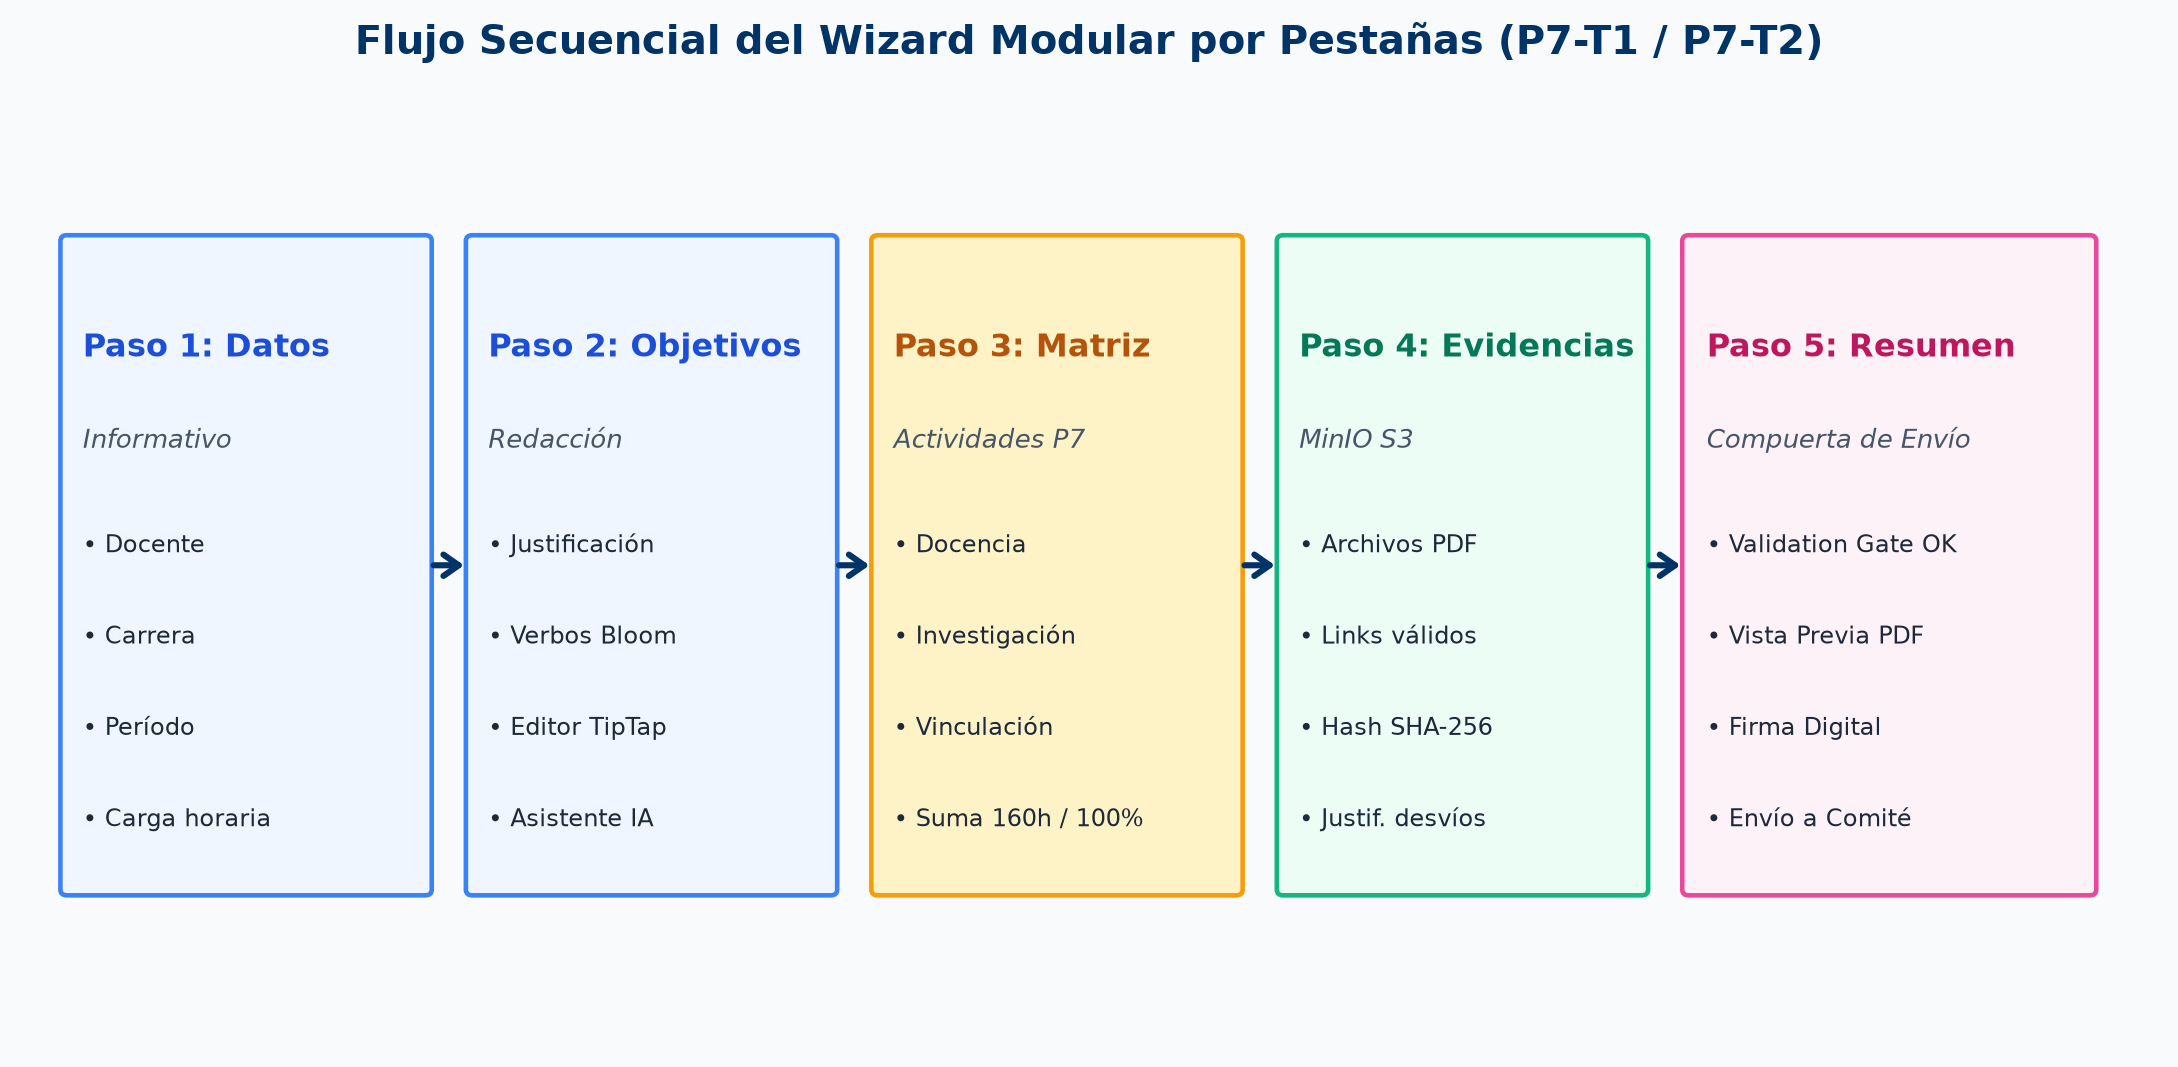
\includegraphics[width=0.88\textwidth,height=5.8cm,keepaspectratio]{images/f3_05_wizard_modular_flujo.png}
    \caption{Flujo Operativo del Asistente Modular (Wizard) en el Plan de Trabajo Docente.}
    \label{fig:anx_f3_05}
\end{figure}

\subsubsection*{Desglose Técnico y Análisis Estructural del Artefacto Visual}
\begin{itemize}[leftmargin=1.5em, itemsep=3pt]
    \item \textbf{Elementos Estructurales Visualizados:} La captura documenta el Asistente Wizard en la Etapa Inicial de configuración. Se aprecia la barra de progreso superior mostrando el 20\% de avance completado, el Stepper con 5 indicadores circulares y el formulario de selección de carrera y carga horaria base (40h).
    \item \textbf{Máquina de Estados y Navegación Reactiva:} Se visualiza el bloqueo declarativo de las etapas subsiguientes (2 a 5): el botón "Siguiente Etapa" permanece inhabilitado hasta que el docente confirme la carrera y el periodo académico activo.
    \item \textbf{Prevención Activa de Errores Cognitivos:} Al desglosar el extenso formulario oficial \texttt{P7- T1} en 5 módulos manejables, el sistema reduce la fatiga visual del docente y elimina el riesgo de omisión de campos requeridos por el SGC.
    \item \textbf{Trazabilidad con el Código Fuente:}\newline Programado en el componente \texttt{frontend/\allowbreak  src/\allowbreak  components/\allowbreak  wizard/\allowbreak  PlanWizard. jsx} y administrado por el hook personalizado \texttt{usePlanWizard. js} con \texttt{useReducer}.
\end{itemize}

\subsection*{Anexo 3: Matriz de Verificación Operacional del Asistente Wizard}
\begin{table}[H]
\centering
\small
\renewcommand{\arraystretch}{1.15}
\begin{tabularx}{\textwidth}{|>{\hsize=0.75\hsize\raggedright\arraybackslash\bfseries\footnotesize}X|>{\hsize=1.25\hsize\raggedright\arraybackslash\footnotesize}X|>{\hsize=1.35\hsize\raggedright\arraybackslash\footnotesize}X|>{\hsize=0.65\hsize\centering\arraybackslash\footnotesize}X|}
\hline
\rowcolor{tableheader}
\textbf{Escenario de Prueba} & \textbf{Condición de Entrada y Acción} & \textbf{Respuesta del Asistente Wizard} & \textbf{Resultado Verificado} \\
\hline
P1: Salto No Autorizado & Clic sobre el icono del Etapa de Evidencias mientras se edita el Etapa Inicial. & Acción interceptada; alerta informativa "Debe completar la matriz de actividades". & Salto Bloqueado \\
\hline
P2: Cierre y Restauración & Recarga completa de pestaña (\texttt{F5}) a mitad del Etapa Descriptiva. & Recuperación automática de todos los textos desde la memoria local. & 0 Pérdida de Datos \\
\hline
P3: Navegación Reversa & Clic en "Etapa Anterior" desde el Etapa Matricial hacia el Etapa Descriptiva. & Transición fluida conservando los datos de la matriz sin alteración. & Retroceso Seguro \\
\hline
P4: Carga Horaria Incorrecta & Ingreso de 35 horas en campo de dedicación de tiempo completo. & Botón "Continuar" deshabilitado; badge en rojo "Se requieren 40h exactas". & Bloqueo Preventivo \\
\hline
\end{tabularx}
\caption{Matriz de pruebas del asistente interactivo modular para la elaboración de planes.}
\end{table}


\end{document}
